\documentclass{scrbook}

\KOMAoptions{%
    fontsize=10pt,          % Tamaño de fuente
    paper=a4,               % Tamaño del papel
    headings=normal,        % Tamaño de letra para los títulos: small, normal,
                            % big
    parskip=full,           % Espacio entre párrafos: full (una línea) o half
                            % (media línea)
    headsepline=false,      % Una linea separa la cabecera del texto
    cleardoublepage=empty,  % No imprime cabecera ni pie en páginas en blanco 
    chapterprefix=false,    % No antepone el texto "Capítulo" antes del número
    appendixprefix=false,	% No antepone el texto "Apéndice" antes de la letra
    listof=totoc,		    % Añade a la tabla de contenidos la lista de tablas 
                            % y figuras
    index=totoc,			% Añade a la talba de contenidos una entrada para 
                            % el índice
    bibliography=totoc,	    % Añade a la tabla de contenidos una entrada para
                            % bibliografía
    BCOR=5mm,               % Reserva margen interior para la encuadernación. 
                            % El valor dependerá el tipo de encuadernado y del
                            % grosor del libro.
    DIV=10,                 % Cálcula el diseño de página según ciertos 
                            % parámetros. Al aumentar el número aumentamos el
                            % ancho de texto y disminuimos el ancho del margen.
                            % Una opción de 14 producirá márgenes estrechos y
                            % texto ancho.
}

% Set input encoding.
\usepackage[utf8]{inputenc}

% Establish Spanish as the default language. English is also used in the
% abstract.
%   es-tabla - Change "Cuadro" for "Tabla".
\usepackage[english, spanish, es-tabla]{babel}

% Set graphics folder path.
\usepackage{graphicx}
\graphicspath{{images/}}

% Enable graphics placement.
\usepackage{float}

% Apply color to tables.
\usepackage{colortbl}

% Set title page background image.
\usepackage{eso-pic}
\newcommand\BackgroundPic{%
	\put(0,0){%
		\parbox[b][\paperheight]{\paperwidth}{%
			\vfill
			\centering
			
\includegraphics[width=\paperwidth,height=\paperheight,%
			keepaspectratio]{ugr/portada-sencilla-color}%
			\vfill
}}}

% Add the euro symbol.
\usepackage{marvosym}
\DeclareUnicodeCharacter{20AC}{\EUR{}}

\usepackage{hyperref}
\usepackage{booktabs}
\usepackage{bookmark}

\begin{document}

\frontmatter
\begin{titlepage}
    \AddToShipoutPicture*{\BackgroundPic}

    \begin{addmargin}[2.575cm]{0cm}
        \begin{flushleft}
            \Large
            \hfill\vfil

            \large{\textsf{Escuela Técnica Superior en Ingenierías Informática y de Telecomunicación}}
            \vfill

            {\large\textsc{Máster Universitario en Ingeniería Informática}} \vfill


            {\large\textsc{trabajo de fin de máster}}

            \begingroup
            \Huge{Título del TFM}
            \endgroup

            \vfill\vfill\vfill\vfill

            \textsf{\normalsize{Presentado por:}}\\
            {\normalsize\textrm{Víctor Vázquez Rodríguez}}
            \bigskip

            \textsf{\normalsize{Tutor:}}\\
            {\normalsize\rmfamily{
                Antonio Javier Díaz Alonso\\
                \emph{Departamento de Arquitectura y Tecnología de Computadores}
            }}

            \bigskip
            \textsf{\normalsize{Curso académico 2020-2021}}
        \end{flushleft}
    \end{addmargin}
\end{titlepage}
\cleardoublepage
\pdfbookmark[1]{Agradecimientos}{Agradecimientos}

\chapter*{Agradecimientos}

Al Dr. Antonio Javier Díaz Alonso, tutor de este trabajo, por guiarme y
aportarme su experiencia académica.

A mis padres, por darme la oportunidad de estudiar y seguir mi propio camino.

Al Dr. Juan Antonio Vázquez Rodríguez, mi hermano, por ser mi referente de
esfuerzo, trabajo, bondad y humildad.

A mi novia, Rosa, por creer siempre en mí y estar a mi lado pase lo que pase.

A mis compañeros de promoción del Máster, por hacerme sentir como en casa lejos
de ella.

\cleardoublepage
\pdfbookmark[1]{Resumen}{Resumen}

\chapter*{Resumen}

\selectlanguage{spanish}
Con el advenimiento de la Industria 4.0, las empresas buscan incorporar técnicas
de inteligencia artificial y análisis de datos a sus instalaciones y procesos
industriales con el objetivo de mejorar la productividad y la autonomía. En este
trabajo, se plantea la posibilidad de usar tecnologías de contenerización de
procesos para el despliegue eficiente de estas nuevas tareas junto con las de
tiempo real habituales en los sistemas de control industrial, estudiando las
distintas tecnologías posibles y realizando un análisis del rendimiento de
tareas de tiempo real contenerizadas con Docker. Además, se diseña e implementa
una herramienta software que sirve como prueba de concepto para el despliegue y
la orquestación de este tipo de tareas sobre entornos distribuidos mediante el
uso de contenedores.

\selectlanguage{english}
\itshape
As Industry 4.0 gets closer, companies are looking to incorporate artificial
intelligence and data analysis techniques to their facilities and industrial
processes with the objective of improving productivity and autonomy. This paper
proposes the use of processes containerization techonologies for efficient
deployment of these new tasks along with the real-time tasks that are common in
industrial control systems, studying different possible techonologies and
analysing the performance of real-time tasks containerized using Docker.
Finally, a proof-of-concept software tool for deployment and orchestration of
this type of tasks on distributed environments by means of containers.

\selectlanguage{spanish}

\cleardoublepage
\pdfbookmark[1]{\contentsname}{toc}

\tableofcontents
\listoffigures
\listoftables
\lstlistoflistings

\cleardoublepage

\mainmatter
\chapter{Introducción}

\section{Motivación y contexto}

El Programma 101 es considerado por muchos como el primer ordenador de uso
personal. Producido por la empresa italiana Olivetti entre los años 1962 y 1964,
este dispositivos seasimilaba más a una calculadora que al concepto de ordenador
que se tiene en la actualidad. Casi 60 años después, los ordenadores han
evolucionado hasta convertirse en un objeto asequible y casi indispensable,
teniendo la mayor parte de la sociedad acceso a algún dispositivo con capacidad
de computación. Aspectos de nuestra vida como el ocio, serían muy diferentes sin
las redes sociales o los servicios online. Esta evolución de los ordenadores y
la computación en general continúa hoy en día, buscando conectar dispositivos
cotidianos a internet e incorporar en ellos cierta capacidad de procesamiento.
Televisores inteligentes en los que instalar aplicaciones, robots aspiradores
que funcionan de manera autónoma, frigoríficos que permiten ver el estado de los
alimentos que almacenan, todos estos productos surgen de la expansión de los
ordenadores hasta todos los rincones de nuestras vidas, con el objetivo final de
hacerla más sencilla para los humanos. Esta expansión no está ocurriendo solo en
los hogares, si no que se avanza hacia un mundo más conectado donde
aparentemente todo lo que nos rodea tenga acceso a la red.

La industria no es ajena a este cambio, ya que la aplicación del internet de las
cosas (IoT por sus siglas en inglés) a los procesos industriales podría aportar
beneficios muy importantes como son el aumento de la productividad, de la
calidad de los productos o de la seguridad de las instalaciones. No obstante, se
trata de un proceso de implantación complejo y de muy largo plazo, debido a los
estrictos requisitos de algunos sectores industriales. Las fábricas y plantas de
producción relegan las tareas de control de sus operaciones a los sistemas de
control industriales o ICSs (\textit{Industrial Control Systems}). Normalmente,
estos sistemas deben responder ante eventos que ocurren en las instalaciones en
ventanas de tiempo muy pequeñas, dependiendo del proceso concreto y sus riesgos
asociados. La fiabilidad de estos sistemas y su tolerancia ante los fallos es de
gran importancia, siendo crucial la verificación de estos aspectos durante su
diseño y desarrollo. Es por estos requisitos tan estrictos que, en muchos casos,
para la implantación de los ICSs se utilizan tanto \textit{hardware} como
\textit{software} específicos y que ya han sido validados para este tipo de
aplicaciones. No obstante, el uso de estas herramientas también plantea algunos
inconvenientes, como por ejemplo la difícil interoperabilidad con otros sistemas
debido a la naturaleza cerrada de las mismas o la reutilización del código en
otras plataformas, lo que acorta la vida útil del \textit{software}.

Desde esta situación se afronta el avance hacia la cuarta revolución industrial
o Industria 4.0. Uno de los objetivos principales que se persigue es la
automatización completa de los procesos industriales, haciando que sean
independientes y autogestionados, aumentando así su eficiencia, productividad y
seguridad. Para conseguir este objetivo, es necesario incorporar a estos
procesos las nuevas técnicas de aprendizaje automático y análisis de grandes
volúmenes de datos, construyendo sistemas experots capaces de tomar decisiones
propias para su funcionamiento y gestión (p. ej., modificar el ritmo de
producción en base a predicciones sobre la demanda). Aunque estos sistemas
expertos se podrían desplegar en plataformas separadas de las que habitan los
ICSs, esto duplica los costes de infraestructura y hace también más difícil el
mantenimiento de la misma. Por ello, hay una tendencia cada vez mayor hacia la
ejecución de tareas con distintos niveles de criticalidad en una misma
plataforma. Por otra parte, las tareas de aprendizaje máquina suelen requerir de
una capacidad de computación relativamente elevada, sobre todo cuando la
cantidad de datos sobre la que se trabaja es grande. Un solo dispositivo no
sería capaz de gestionar estas tareas de forma eficiente si, además, debe
realizar tareas críticas de control, dificultando también que pueda cumplir con
sus requisitos en ese aspecto. Aparecen entonces nuevos paradigmas de
computación, como el \textit{fog} o el \textit{edge computing}, que pretenden
decentralizar el procesamiento, alejándolo de la nube y llevándolo a elementos
intermedios más cercanos a las fuentes de datos o a los dispositivos del borde
de la red, respectivamente. En estos paradigmas, se persigue la máxima
utilización de la capacidad de computación de los dispositivos presentes en la
red, distribuyendo entre ellos las tareas necesarias de forma dinámica.

Dentro de este campo, se están llevando a cabo muchas investigaciones para
validar la efectividad de estos nuevos modelos y hacerlos realidad, además de
comprobar su efectividad en el ámbito industrial. Uno de los planteamientos más
prometedores es el que conlleva la aplicación de tecnologías de virtualización a
los sistemas de control industrial, permitiendo su despliegue y ejecución
distribuida en convivencia con otros procesos. Estas tecnologías, que han
sufrido un desarrollo masico en los últimos años debido al auge de la
computación en la nube, pueden ahora ser claves para asegurar la resiliencia y
robustez de los ICSs en entornos distribuidos.

Por todo esto, este trabajo abordará la complejidad de los problemas descritos
intentando buscar mecanismos que simplifiquen la gestión de los sistemas
\textit{fog}/\textit{edge}. Partiremos de la experiencia previa en trabajos con
contenedores orientados al análisis de sus prestaciones para la ejecución de
tareas con restricciones temporales, responsables de las ideas aquí propuestas y
base fundamental de parte de la motivación de este trabajo. Además, esta línea
de investigación tiene mucho potencial para mejorar los sistemas de control
implementados en la actualidad, permitiendo por tanto una contribución
importante tanto en aspectos industriales como científicos, lo que aumenta aún
más nuestro interés en esta temática.

\section{Objetivos}

De cara a la realización de este trabajo, se han planteado los siguientes
objetivos a cumplir:

\begin{itemize}
    \item Comprender los conceptos básicos sobre sistemas operativos de tiempo
          real, algoritmos de planificación y sistemas de control industriales.
    \item Analizar las soluciones de tiempo real basadas en GNU/Linux existentes.
    \item Estudiar la viabilidad y rendimiento de las tecnologías de
          contenerización para la ejecución de tareas con restricciones temporales.
    \item Diseñar e implementar una herramienta de despliegue de tareas de
          tiempo real mediante contenedores que sirva como prueba de concepto.
    \item Caracterizar las prestaciones de la herramienta desarrollada,
          identificando posibles aplicaciones y/o mejoras de la misma.
\end{itemize}

Una parte relevante de los objetivos del presente proyecto están asociados al
estudio y caracterización de tecnologías, así como al análisis del mercado, que
se justifica por un enfoque innovador orientado al desarrollo de sistemas para
\textit{fog computing}. Esto, junto con los conocimientos adquiridos sobre
implementación de sistemas de tiempo real, será clave para que la herramienta
desarrollada como prueba de concepto sea lo más eficiente y funcional posible.

Por otra parte, en los objetivos también se hace hincapié en el uso de
soluciones basadas en GNU/Linux, como parte de un fuerte compromiso con las
herramientas libres y de código abierto. Algunos de los sistemas operativos de
tiempo real más conocidos y usados son de código propietario y es necesario
adquirir licencias para utilizarlos, lo cual no favorece ni el aprendizaje ni la
reutilización del software desarrollado para estas plataformas. Últimamente, se
han realizado contribuciones importantes al kernel de Linux para mejorar el
soporte que ofrece a cargas de trabajo de este tipo, además de los múltiples
proyectos más especializados que está llevando a cabo la comunidad. En esta
aproximación, hemos considerado primordial la extensión del software libre,
apoyando su uso siempre que sea posible. Por ello, la herramienta planteada se
diseñará en torno al despliegue de tareas en sistemas GNU/Linux.

\section{Planificación}

\section{Material y métodos}

En esta sección, se presentan todas las herramientas que se han usado para
llevar a cabo este proyecto, además de las metodologías de trabajo seguidas. En
la figura \ref{fig:01-tools} se puede ver una recopilación de los logotipos de
todas estas herramientas, las cuales se van a exponer en detalle a continuación.

En un proyecto de desarrollo de código como es este, una de las herramientas más
importantes es la de control de versiones. En nuestro caso, se ha usado
\textbf{Git} debido a que es una herramienta de código libre y, además, es la
más conocida y usada. El repositorio remoto se ha alojado en \textbf{GitHub}, la
popular plataforma de desarrollo de código colaborativo. El desarrollo de código
como tal se ha hecho con \textbf{Visual Studio Code}, un editor de texto de
Microsoft que, aunque ofrece menos funcionalidad de serie que los entornos de
desarrollo (IDEs) especializados, también es mucho más liviano y rápido. Además,
esta funcionalidad se puede extender enormemente mediante extensiones, pudiendo
convertirlo casi en un IDE adaptado a las necesidades concretas del usuario.
Gracias a estas extensiones, se puede usar el mismo editor para distintos
programar en distintos lenguajes, lo cual ha sido una de las principales razones
por las que se ha escogido.

Como ya se ha indicado en la sección anterior, se ha aplicado un SCRUM adaptado
como metodología de planificación, gestión y seguimiento del proyecto, usando un
tablero Kanban para la visualización de las tareas. Concretamente, se ha usado
el tablero que ofrece GitHub como parte de sus herramientas para la gestión de
proyectos. Las tareas se añaden a los repositorios como \textit{issues}, los
cuales se añaden al tablero para controlar su estado de realización. El
beneficio que nos aporta el uso de GitHub para esto es el de tener una
plataforma unificada tanto para la gestión del proyecto como para su desarrollo.
Esta integración permite flujos de trabajo muy interesantes, como por ejemplo
referenciar los \textit{issues} ya mencionados en los mensajes de
\textit{commit}, de forma que se vinculan los cambios realizados con la tarea en
la que se engloban. La gestión del proyecto es, por tanto, más directa y
sencilla.

\textbf{Incorporar imagen del tablero del proyecto de GitHub}

Los diagramas que se presentan a lo largo de este trabajo, incluidos los que
componen el diseño de la herramienta desarrollada y sus componentes, se han
creado con la herramienta online \textbf{draw.io}. Al integrarse directamente
con Google Drive, se puede usar desde el navegador, siendo una solución muy
cómoda y accesible para la creación de estos diagramas.

En cuanto al desarrollo y despliegue de la herramienta planteada, se han
utilizado varias tecnologías. Los lenguajes de programación son Python y C, muy
conocidos y utilizados en la industria. C es el lenguaje de referencia para la
programación de sistemas y las tareas de bajo nivel, mientras que Python ofrece
una sintaxis muy sencilla para la implementación de herramientas como
aplicaciones o servidores. Python también posee una nutrida colección de
librerías para distintos casos de uso, lo cual también fue muy atractivo para su
elección. En este proyecto, se usan varias de estas librerías para facilitar la
implementación de algunos aspectos de la herramienta. Destacamos las siguientes:

\begin{itemize}
    \item \textbf{hug} - Escritura de APIs sencilla y sin ataduras. Esta
          librería trata de competir con otras más conocidas como Flask, proponiendo
          un modelo mucho más simple y dando más libertad al desarrollador.
    \item \textbf{click} - Más que una librería, se trata de un
          \textit{framework} para la implementación de aplicaciones de línea de
          comandos (CLI). Ofrece todas las utilidades que se pueden necesitar para
          este tipo de aplicaciones, como es la generación automática de páginas de
          ayuda.
    \item \textbf{marshmallow} - Esta librería permite la sencilla
          deserialización y serialización de objetos JSON a objetos Python. Esto es
          especialmente útil al trabajar con servicios web, ya que se pueden leer los
          datos JSON recibidos y validarlos frente a un esquema de datos definido por
          el desarrollador.
    \item \textbf{pymongo} - Ejecución de consultas sobre bases de datos
          MongoDB, que son las usadas en este proyecto.
    \item \textbf{paramiko} - Herramientas para trabajar con SSH desde Python.
          Esencial para el despliegue de las tareas sobre los nodos.
    \item \textbf{docker} - La librería oficial de Docker para Python. Con ella,
          se puede conectar con un servidor Docker (local o remoto) para ejecutar
          operaciones de construcción de imágenes o lanzamiento de contenedores.
    \item \textbf{requests} - Es la librería más conocida para la realización de
          peticiones HTTP en Python.
    \item \textbf{unittest} - Aunque no se trata de una librería externa como
          las demás, ya que forma parte de la librería estándar de Python, merece ser
          destacada por ser la utilizada para la escritura y ejecución de las pruebas
          del código desarrollado.
\end{itemize}

Además de estas librerías, se han usado otras para el análisis y formateo del
código como son \textbf{pylint} y \textbf{autopep8}.

Como ya se ha mencionado, la herramienta desarrollada trabaja con
\textbf{MongoDB} para la gestión del almacenamiento persistente de los datos y
el acceso a los mismos. Se trata de un gestor de bases de datos documental que
pertenece a la familia NoSQL (\textit{Not only SQL}). Las bases de datos
documentales divergen del modelo relacional tradicional que siguen otros
gestores tan famosos como MySQL o PostgreSQL. No existen los conceptos de tabla
o fila, sino que se almacenan colecciones de documentos no estructurados. En el
caso de MongoDB, se trabaja con documentos JSON, formato ampliamente usado en el
entorno web para la transmisión de datos debido a su legibilidad y velocidad de
serialización/deserialización. Cuando decimos que los documentos son no
estructurados, nos referimos a que no tienen por qué poseer los mismos campos,
ya que no hay un esquema definido a seguir. MongoDB no cumple con ACID, pero es
una pérdida aceptable a cambio de la flexibilidad y facilidad de uso que nos
ofrece. Además, el lenguaje de consultas es mucho más claro e intuitivo que SQL,
permitiendo realizar consultas de envergadura similar.

\begin{figure}[H]
    \centering
    
\includegraphics[width=0.7\textwidth]{01-introduction/tools.png}
    \caption{Logotipos de las herramientas utilizadas. De izquierda a derecha y%
        de arriba a abajo: Python, Docker, Raspberry Pi, GitHub, VS Code y
        draw.io}
    \label{fig:01-tools}
\end{figure}

La idea principal en torno a la cual gira este trabajo es la del uso de
contenedores para el despliegue de tareas de tiempo real. En este sentido,
\textbf{Docker} es la tecnología de contenerización en la que nos hemos apoyado
para la implementación de la herramienta propuesta. Esta elección recae
principalmente en el hecho de que se trata del motor de contenedores más
conocido y utilizado. De la mano de Docker, también se ha utlizado
\textbf{Docker Compose} para el despliegue sencillo de un entorno de desarrollo
completo que permita replicar un despliegue de producción de forma simplificada.
Las imágenes de contenedores definidas en este proyecto, se han alojado en el
repositorio de imágenes \textbf{DockerHub}, aprovechando que proporciona un
sistema de construcción automática de imágenes.

Para realizar las pruebas del sistema desarrollado, se ha usado una
\textbf{Raspberry Pi 4B}, concretamente la que se muestra en la figura
\ref{fig:01-raspberry-pi}. Se trata de un SBC (\textit{Single Board Computer})
de bajo coste y muy versátil, pudiendo usarse para infinidad de aplicaciones.
Las características detalladas de esta plataforma se pueden ver en la tabla \ref{tab:01-raspberry-specs}.

\begin{table}[H]
    \centering
    \begin{tabular}{ |>{\columncolor[gray]{0.8}}l|p{0.5\textwidth}| }
        \hline
        \textbf{Procesador}          & Cortex-A72                \\
        \hline
        \textbf{Arquitectura}        & ARMv7                     \\
        \hline
        \textbf{Número de núcleos}   & 4                         \\
        \hline
        \textbf{Frecuencia de reloj} & 1500 MHz                  \\
        \hline
        \textbf{RAM}                 & 4 GB                      \\
        \hline
        \textbf{Sistema operativo}   & Raspberry Pi OS Lite 4.19 \\
        \hline
    \end{tabular}
    \caption{Especificaciones de la Raspberry Pi usada en el trabajo}
    \label{tab:01-raspberry-specs}
\end{table}

El sistema operativo de este dispositivo es GNU/Linux (concretamente, basado en
Debian), y se le ha aplicado la revisión 24 del parche de tiempo real
\textbf{PREEMPT-RT}. Este parche aporta al sistema la capacidad de realizar
planificación de procesos apropiativa.

\begin{figure}
    \centering
    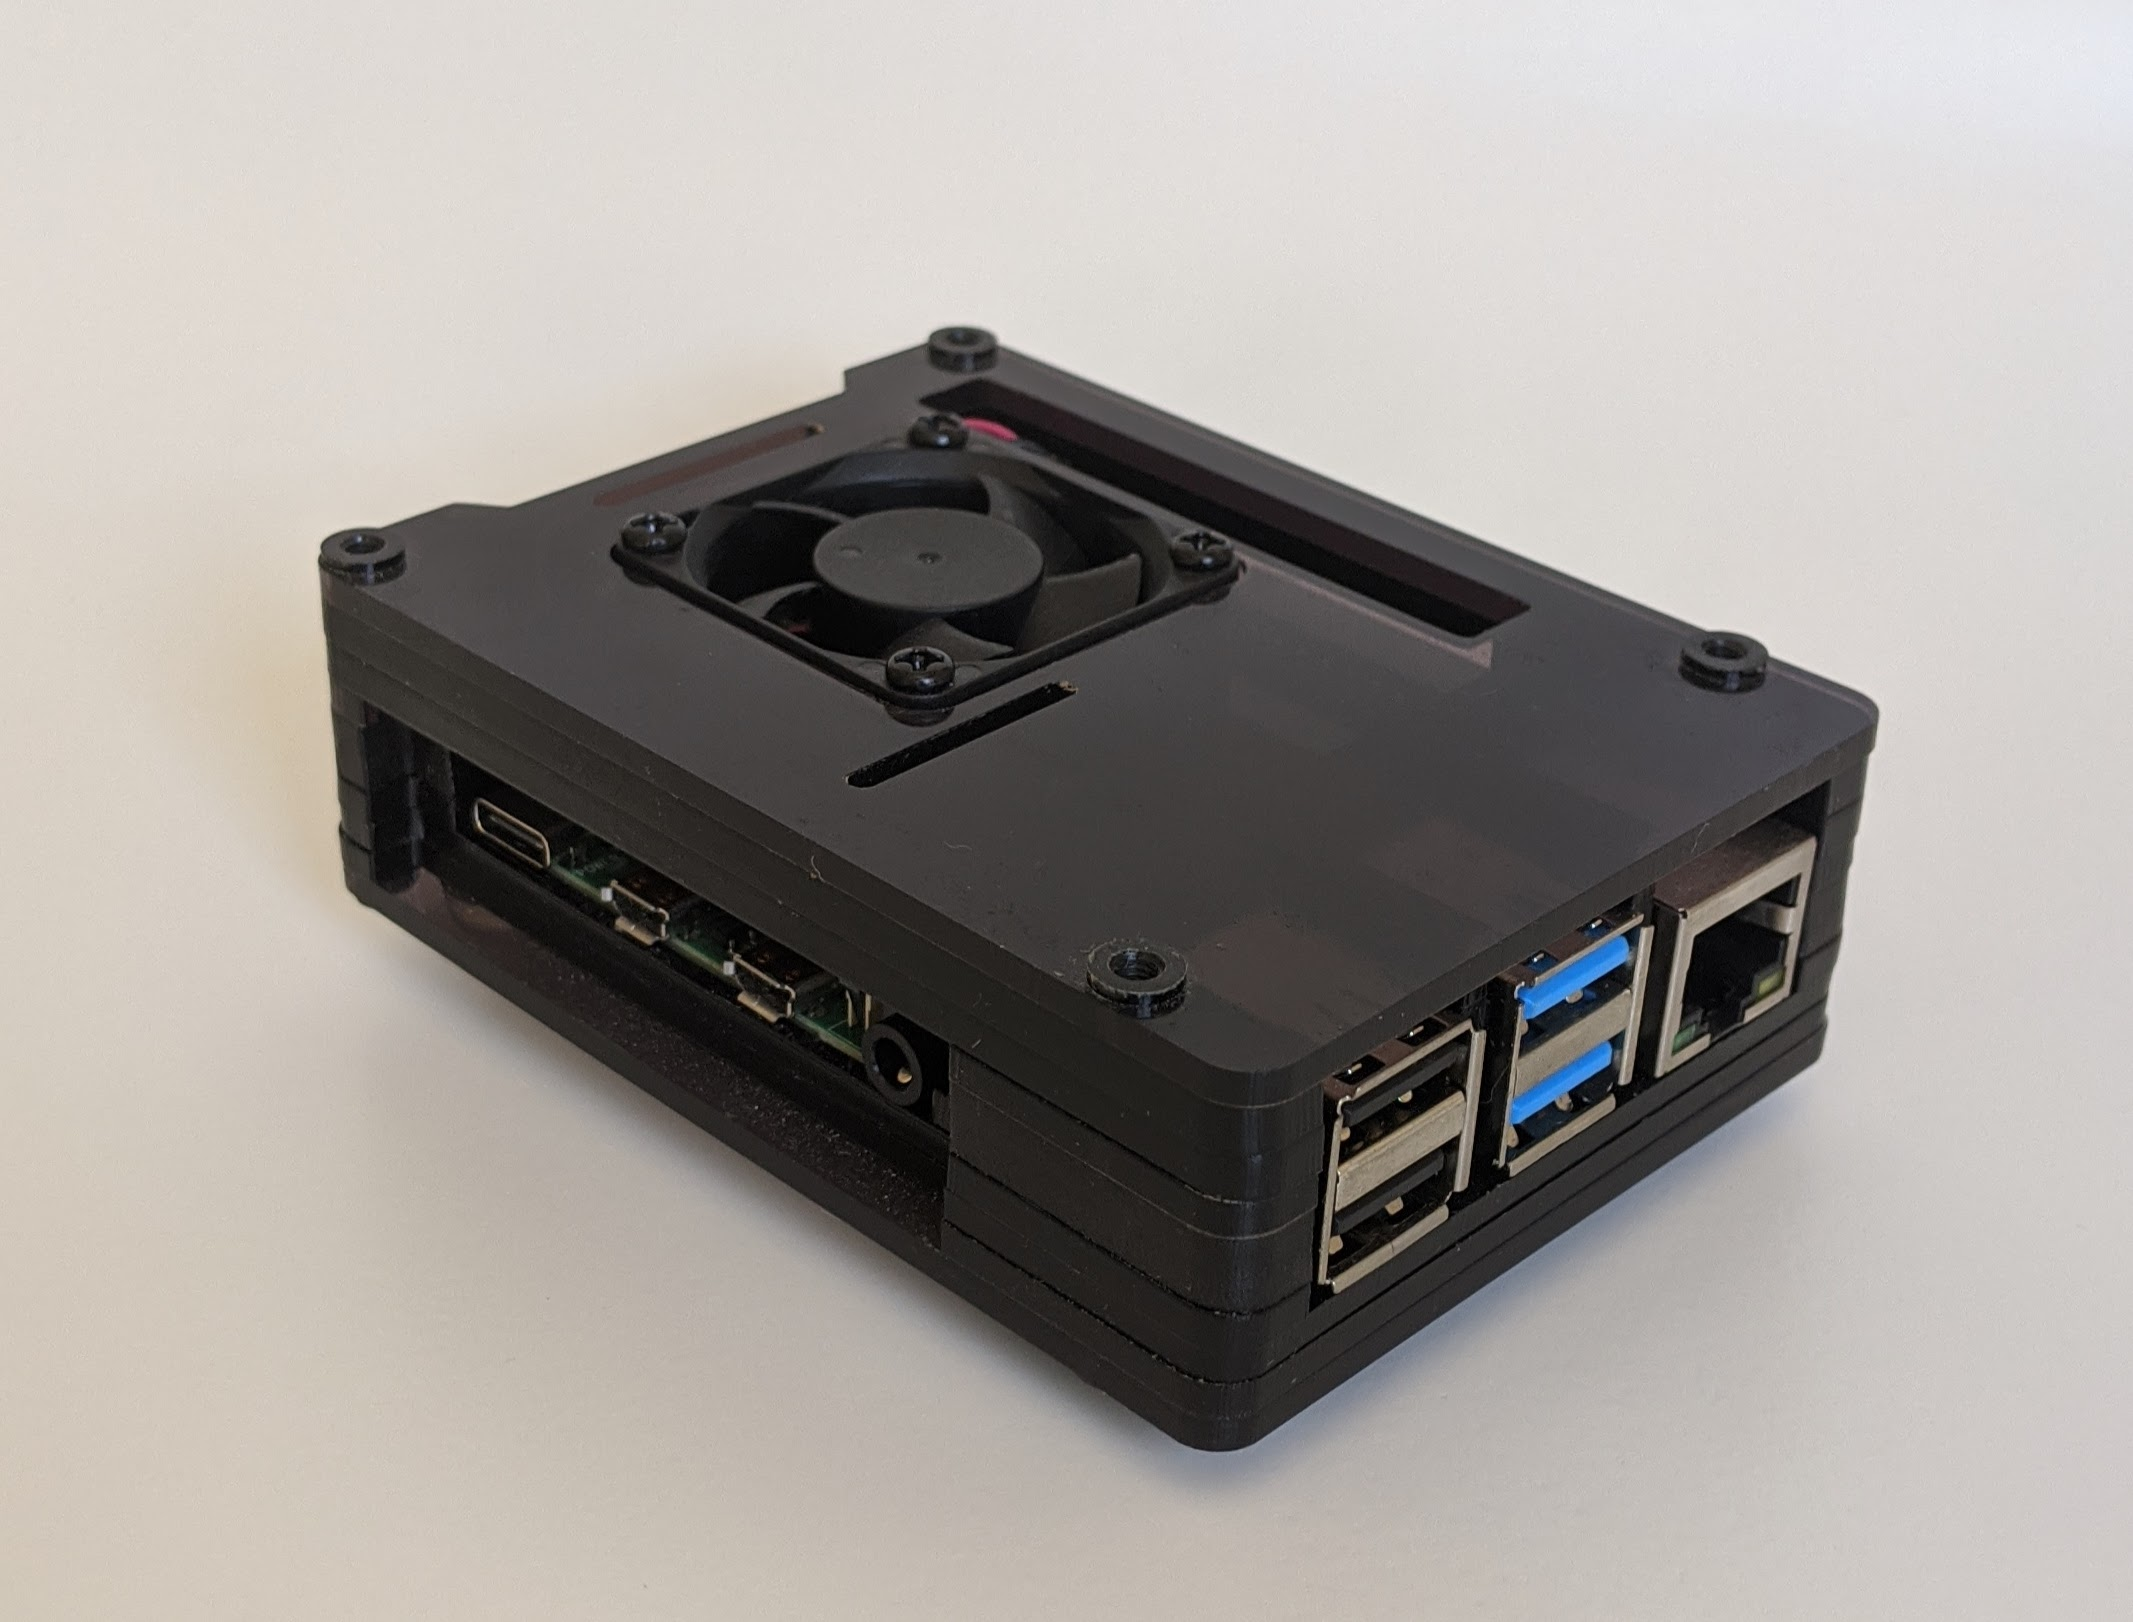
\includegraphics[width=0.8\textwidth]{01-introduction/raspberry-pi.jpg}
    \caption{Raspberry Pi 4B utilizada en el trabajo}
    \label{fig:01-raspberry-pi}
\end{figure}

\section{Estructura de la memoria}

La estructura de la presente memoria es la siguiente:

En el capítulo 1, se ha introducido el proyecto y explicado tanto la motivación
detrás del mismo como los objetivos planteados, la planificación seguida y las
herramientas, tecnologías y metodologías que se han utilizado.

En el capítulo 2, se realiza un estudio en profundidad del estado de la técnica
en lo relativo a los sistemas confiables, las tareas de tiempo real y las
tecnologías de virtualización. Se presentan otros estudios interesantes llevados
a cabo en esta área y se introducen todos los conceptos relevantes.

En la sección 3, se aborda el diseño de una herramienta para el despliegue y
seguimiento de tareas de tiempo real en entornos distribuidos, así como su
implementación y prueba. Se presentan los resultados obtenidos y se discute
sobre los mismos.

En la sección 4, se realiza una revisión del proyecto completo y se presentan
las conclusiones, así como las maneras en las que se puede extender y mejorar el
trabajo realizado.


\appendix
\pdfbookmark[-1]{Apéndices}{appendix}
\chapter{Estimación de costes del proyecto}

Al tratarse, mayoritariamente, de un proyecto de Ingeniería del Software, se ha
realizado también una estimación de los costes asociados a la realización del
mismo. Para ello, se ha aplicado un modelo basado en tiempo y materiales. En
2019, el coste salarial medio de un ingeniero informático recién salido de la
universidad en España era de entre 24.000 y 28.500 euros brutos al año. En esta
estimación, se ha asumido un salario mensual de 2.000€ brutos al mes, que es
aproximadamente un salario anual de 24.000€. Las tareas de coordinación y
dirección del jefe del proyecto se estiman en un 10\% del trabajo de ingeniería,
con un coste medio mensual de unos 5.000€ al mes para un ingeniero sénior.
Además, se ha supuesto también una jornada laboral que llega al máximo en España
de 40 horas semanales. También se tiene en cuenta el coste del hardware usado
para pruebas. La estimación final del coste de desarrollo de este proyecto se
muestra en la tabla \ref{tab:A1-costs}.

\begin{table}[H]
    \centering
    \begin{tabular}{ | >{\columncolor[gray]{0.8}}l | p{0.2\textwidth} r | }
        \hline
        Raspberry Pi 4B 4GB         &  & 60,00€     \\
        \hline
        Cable Ethernet              &  & 7,00€      \\
        \hline
        Cable de alimentación USB-C &  & 7,00€      \\
        \hline
        Mano de obra ingeniero      &  & 8.000,00€  \\
        \hline
        Mano de obra ingeniero jefe &  & 20.000,00€ \\
        \hline
        \multicolumn{1}{ r |}{}     &  & 28.074,00€ \\
        \cline{2-3}
    \end{tabular}
    \caption{Desglose de costes del proyecto}
    \label{tab:A1-costs}
\end{table}

A todo esto habría que sumarle el coste de la estación de trabajo usada para el
desarrollo del proyecto, la cuál consiste de un ordenador de sobremesa o
portátil y los periféricos necesarios, junto con los gastos asociados al consumo
eléctrico y el acceso a internet. Estos gastos se han omitido de la estimación
realizada debido a que son muy variables y tampoco tienen un impacto muy
representativo en los costes del proyecto.


\backmatter
%\bibliographystyle{ieeetr}
%\bibliography{sources}

\end{document}